\chapter{Xây dựng UIT-OWL Editor}
\paragraph{Giới thiệu} Qua các chương trước, chúng em đã trình bày các cơ sở lý thuyết từ Semantic Web, Ontology Web Language và giới thiệu khái quát về OWL-API, Vaadin Framework- 2 công cụ chính xây dựng nên ứng dụng chỉnh sửa và phát triển Ontology trên Web mà chúng em tạm gọi là UIT-OWL Editor. Trong chương này, chúng em sẽ trình bày một cách chi tiết nhất có thể về quá trình xây dựng và phát triển nên ứng dụng này.
\section{Bố cục của ứng dụng}
\begin{figure}[h!]
	\centering
	\frame{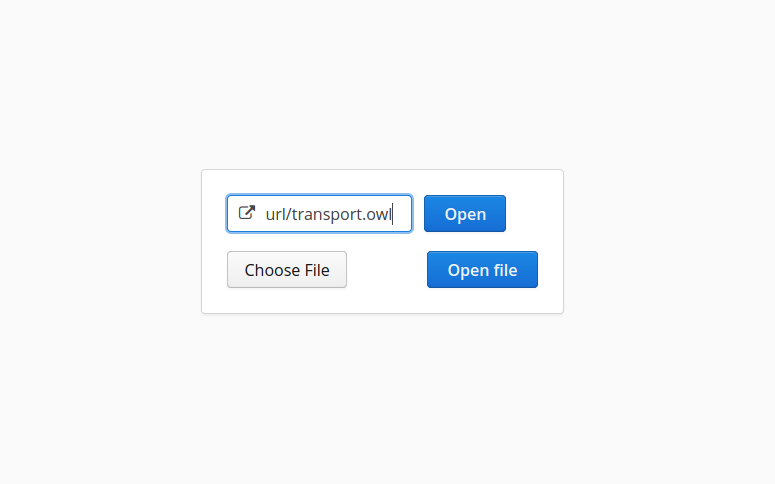
\includegraphics[width=100mm]{Figures/owleditor_entryview.png}}
	\caption{EntryView của UIT-OWL Editor\label{overflow}}
\end{figure}
\begin{figure}[h!]
	\centering
	\frame{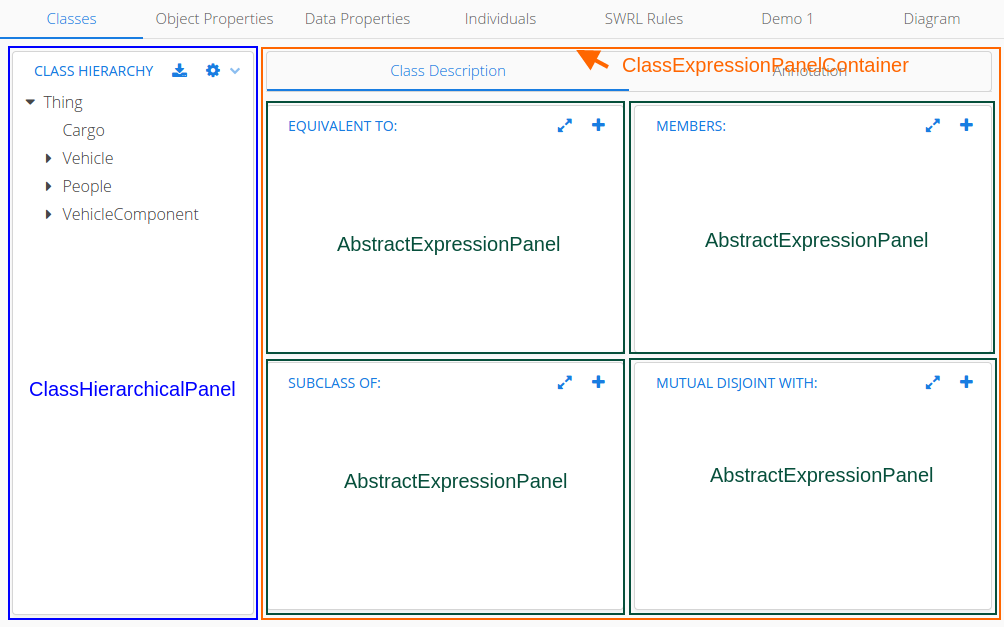
\includegraphics[width=150mm]{Figures/owleditor_mainview.png}}
	\caption{MainView của UIT-OWL Editor\label{overflow}}
\end{figure}
Ứng dụng UIT-OWLEditor chỉ gồm 2 View chính:
\begin{description}
\item[Entry View] tương đương với lớp \textit{vn.edu.uit.owleditor.EntryView} trong mã nguồn, là nơi chúng tập nhập vào URL của file OWL2 Ontology hoặc tải file OWL2 Ontology với các định dạng được trình bày trong chương 2.
\item[Main View] tương đướng với lớp \textit{vn.edu.uit.owleditor.MainView} trong mã nguồn,
là giao diện chính của ứng dụng UIT-OWL Editor, cung cấp những tính năng can thiệp vào thành phần của OWL 2 Ontology đã đề cập trong chương 2.
\end{description}

\section{Cấu trúc package của ứng dụng}
\subsection{vn.edu.uit.owleditor}
Chứa các đối tượng có vai trò là nơi đầu tiên code được thực thi khi người dùng gõ vào URL của ứng dụng. Gồm các đối tượng quan trọng sau
\begin{description}
\item[OWLEditorUI] là đối tượng được mở rộng (thừa kế) lớp \verb|UI| của Vaadin với chứng năng là nạp các component từ Entry 
\end{description}